\newpage
\section*{Geometric atlas of the overlap nerve}
The following plates show the complete exported overlap-nerve 2-skeletons,
with identical connectivity in oblique and overhead views.
Each vertex represents an object of the face poset: a witnessed index set
$\sigma\in K_W^{(2)}$. Circles, squares and triangles distinguish
$|\sigma|=1,2,3$; all three marker types are vertices of the categorical nerve.
An edge represents a strict inclusion $\sigma\subset\tau$.
A filled triangular face represents a composable chain
$\sigma\subset\tau\subset\upsilon$ and includes the composite edge
$\sigma\subset\upsilon$. Line direction is suppressed for visual clarity;
inclusion always points from the smaller to the larger index set.

\begin{figure}[H]\centering
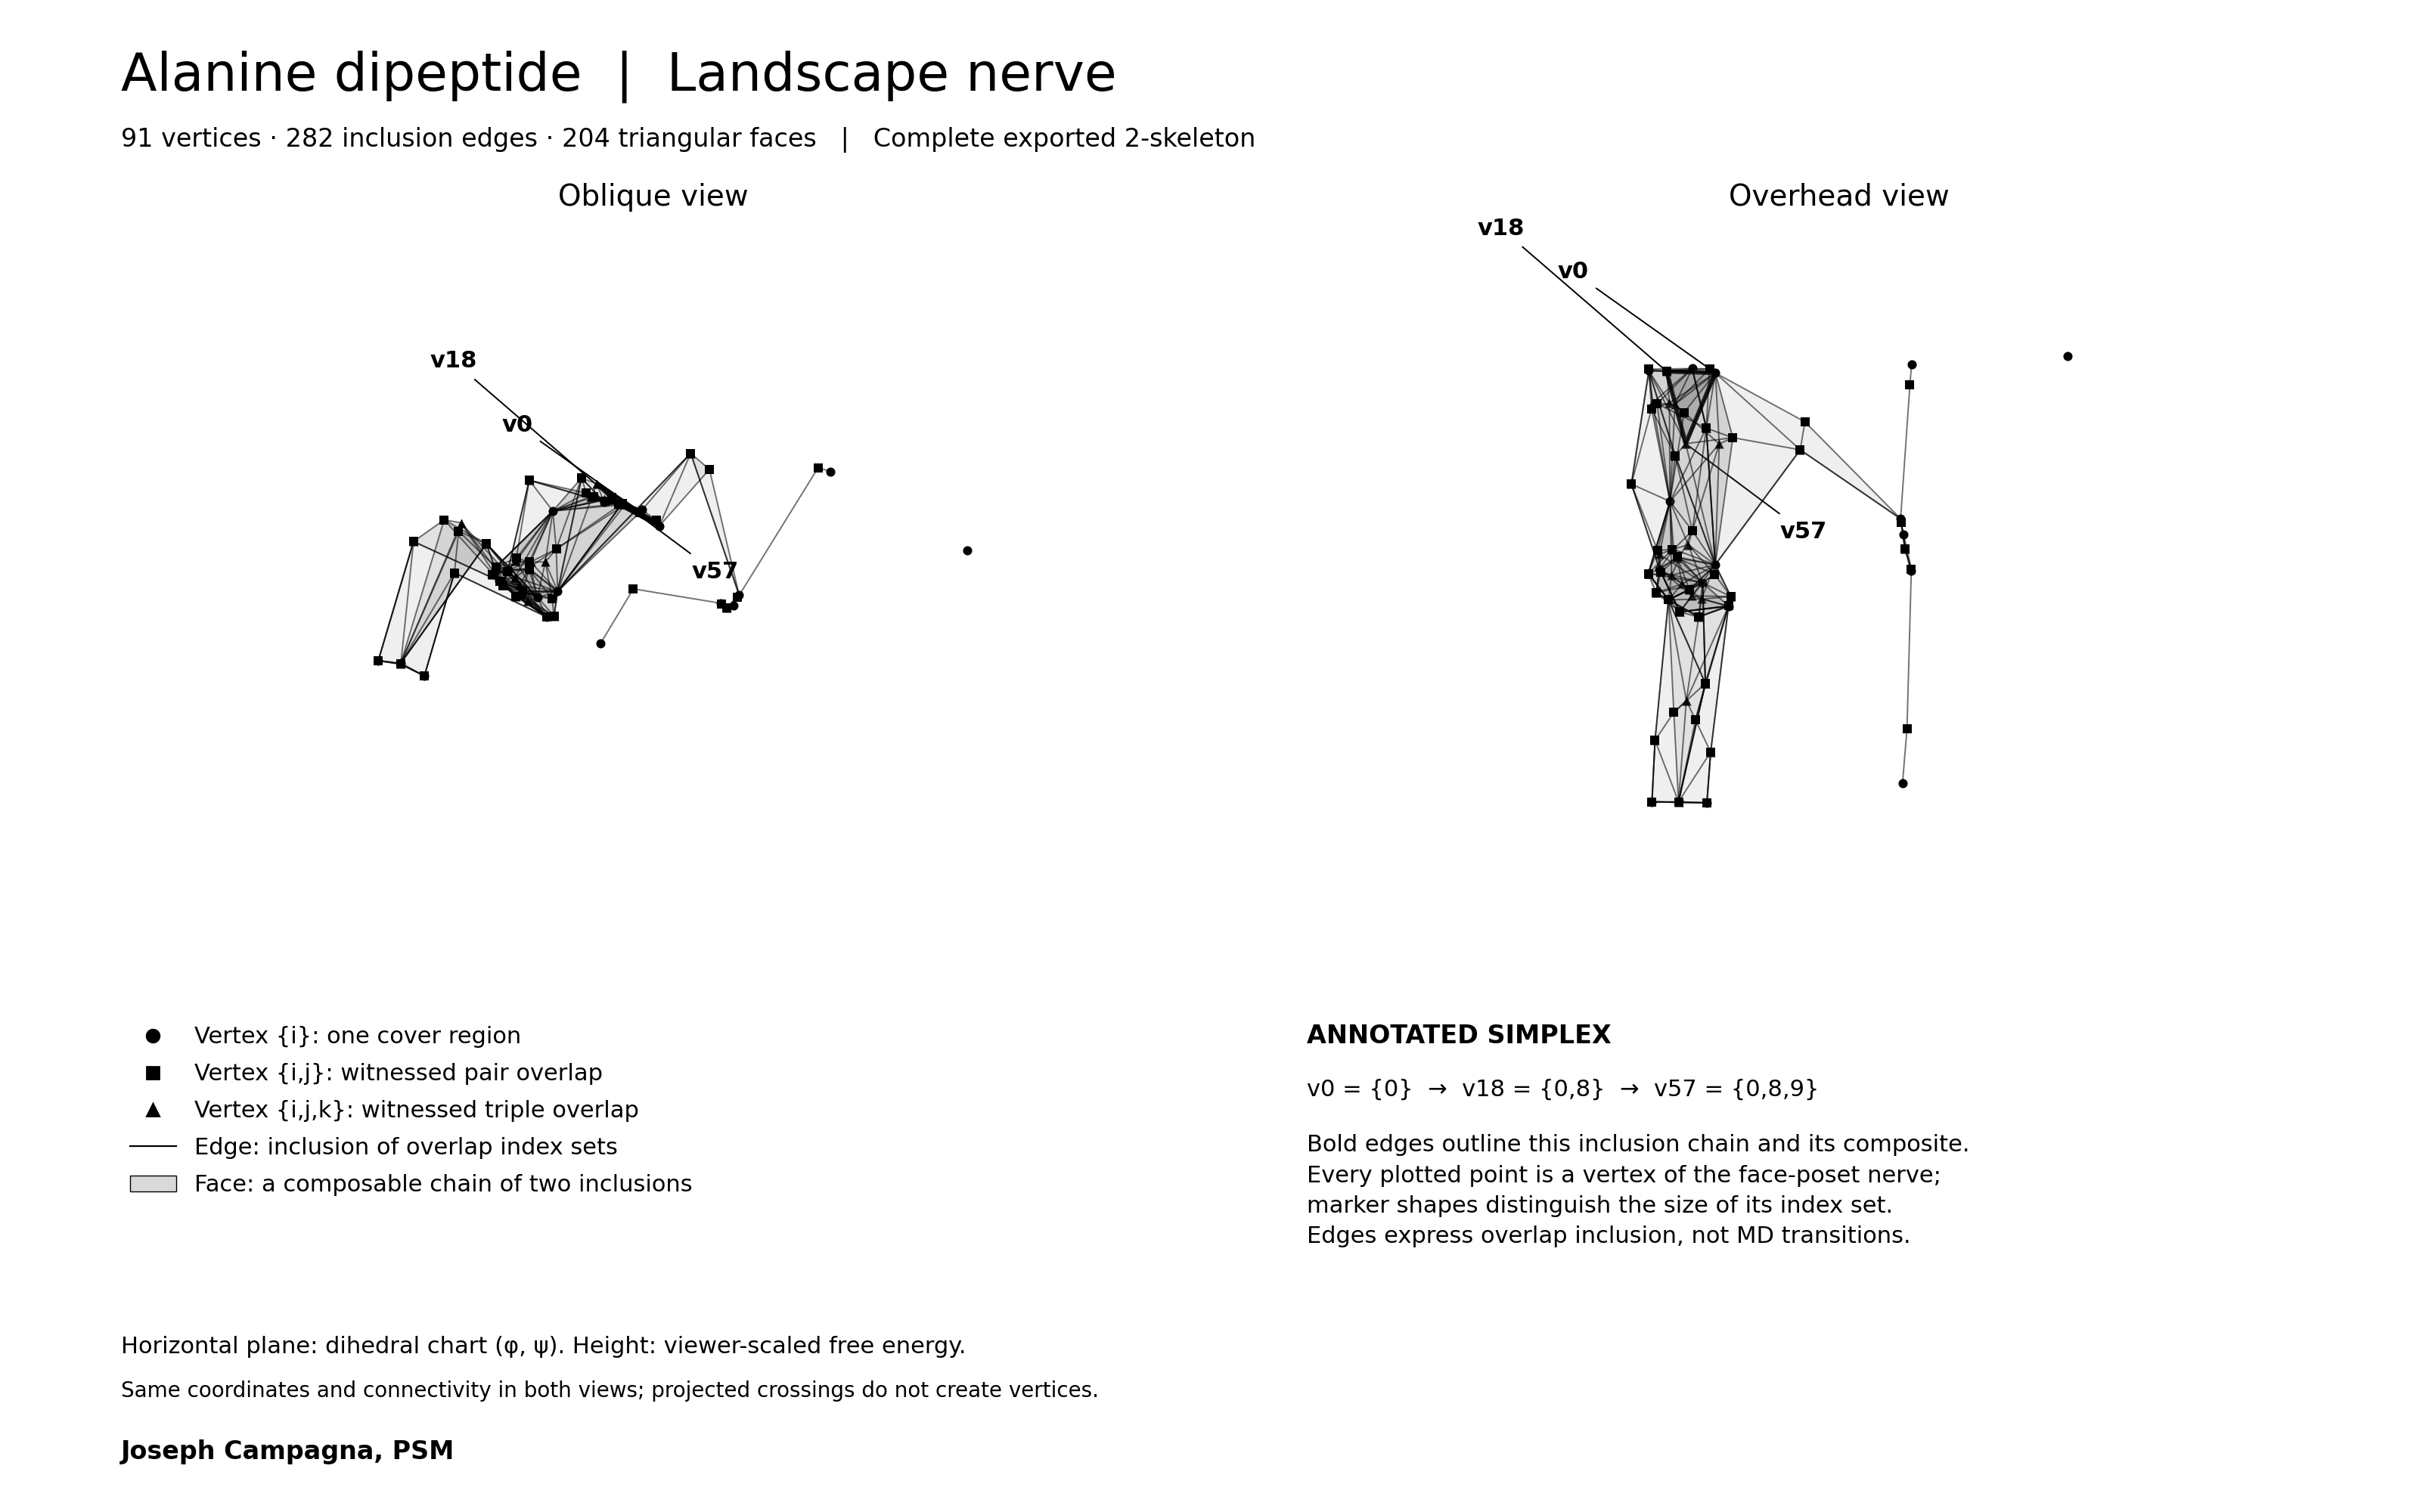
\includegraphics[width=\linewidth]{figures/alanine-nerve-annotated-both.png}
\caption{\textbf{Alanine: the full exported overlap nerve in two views.}
All 91 vertices, 282 strict inclusion edges and 204 triangular faces are
displayed. The labeled example is
$v_0=\{0\}\subset v_{18}=\{0,8\}\subset v_{57}=\{0,8,9\}$.
Vertex IDs are zero-based indices in the exported node array.
Horizontal coordinates follow the viewer's cut $(\phi,\psi)$ chart;
height follows its scaled empirical free-energy coordinate.
The shape is an embedding of the exported combinatorics, not a reconstructed
physical molecular surface.}
\end{figure}
The vertex positions are recorded representatives of the corresponding overlaps,
not necessarily geometric barycenters. Thus the displayed linear triangles
can cross or overlap in projection. These crossings do not create new vertices
or alter the abstract nerve. The categorical realization statement above
concerns the abstract complex, not an injective embedding in this chart.

\newpage
\section*{Geometric atlas of the CLN025 overlap nerve}
\begin{figure}[H]\centering
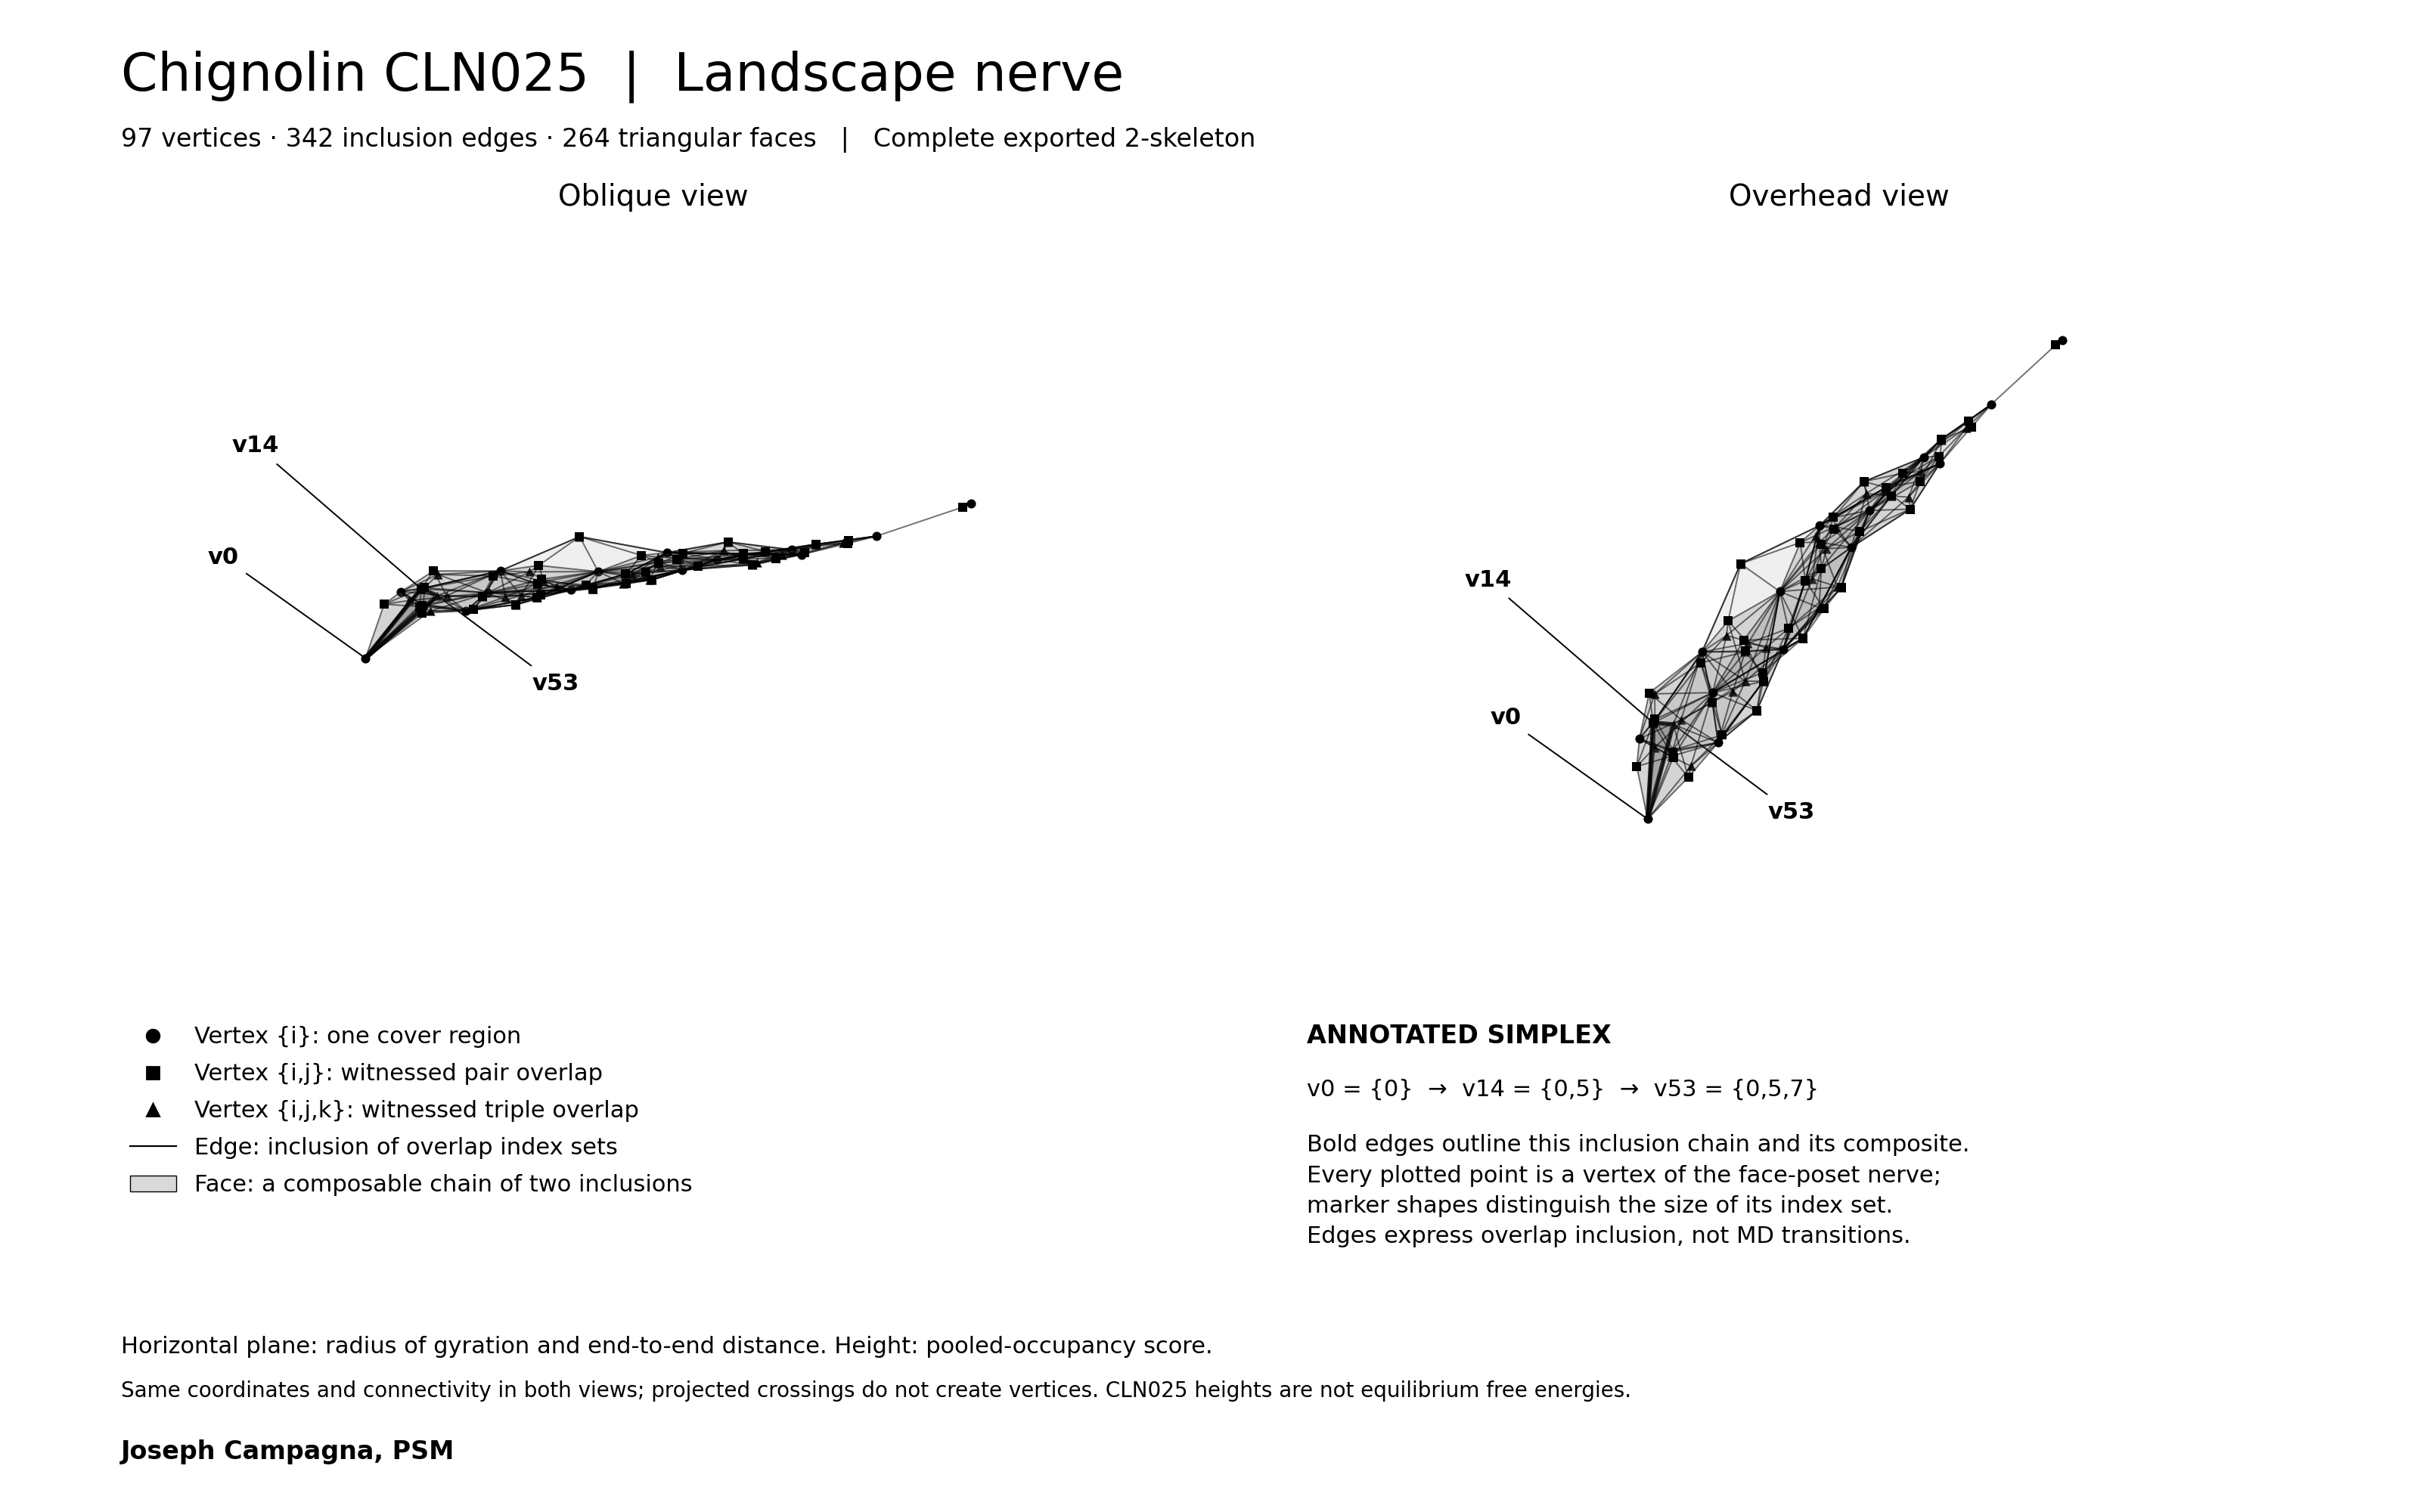
\includegraphics[width=\linewidth]{figures/chignolin-nerve-annotated-both.png}
\caption{\textbf{CLN025: the full exported overlap nerve in two views.}
All 97 vertices, 342 strict inclusion edges and 264 triangular faces are
displayed. The labeled example is
$v_0=\{0\}\subset v_{14}=\{0,5\}\subset v_{53}=\{0,5,7\}$.
The horizontal chart uses C$\alpha$ radius of gyration and end-to-end
distance. Vertical placement follows the viewer's pooled-occupancy score;
it is not an equilibrium free-energy estimate. Marker and edge conventions
match the alanine plate.}
\end{figure}
The elongated geometry reflects the chosen observables and sampled
conformations. It does not establish a folding reaction coordinate or a
topological equivalence with configuration space. The displayed edges are
overlap inclusions, not kinetic pathways; the free path-category overlay
remains a separate construction.

\textbf{Reproducing the plates.}
Run \texttt{python paper/render\_annotated\_nerve.py} from
\texttt{alanine-nerve/}. The script reads the exported node positions,
inclusion edges and chains directly, writes the paired plates into
\texttt{paper/figures/}, and also exports individual viewpoints and SVG
versions into the repository's \texttt{output/nerve-diagrams/annotated/}
directory. No connectivity is inferred from the rendered image.
